\documentclass[preview]{standalone}

\usepackage{tikz}
\usepackage{pgfplots}


\begin{document}
	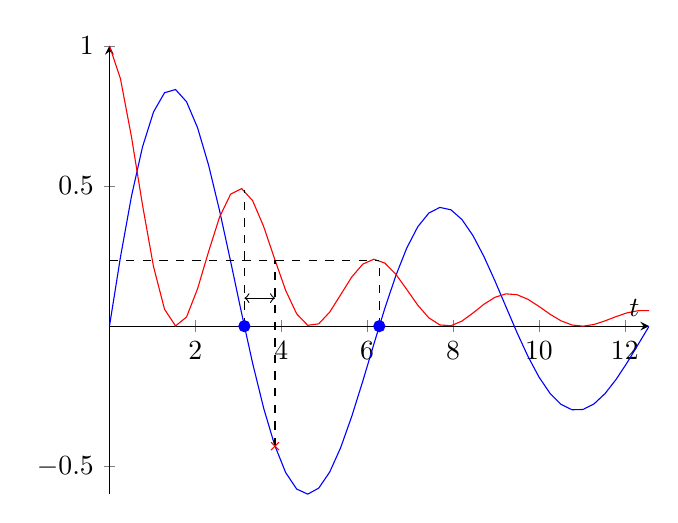
\begin{tikzpicture}
	\begin{axis}[axis lines=center, xlabel=$t$, domain=0:4*pi, legend pos=outer north east,
	declare function ={
		signal(\x) = exp(-.11*\x)*sin(deg(\x));
		info(\x) = exp(-.23*\x)*cos(deg(\x))^2;
	},
	samples=50
]
	\addplot[blue] {signal(x)}; %\addlegendentry{signal}
	\addplot[red] {info(x)}; %\addlegendentry{$f(t_i)$}
	\addplot[mark=none,dashed, domain=0:2*pi]{.2357};
	\draw[dashed] (axis cs:2*pi,0) -- (axis cs:2*pi,{.2357});
	\addplot[mark=*, color=blue] coordinates {(2*pi,0)};
	\draw[dashed] (axis cs:3.8547,-.4281) -- (axis cs:3.8547,{.2357});
	\addplot[mark=*, color=blue] coordinates {(pi,0)};
	\addplot[mark=x,color=red] coordinates {(3.8547,-.4281)};
	\draw[dashed] (axis cs:pi,0) -- (axis cs:pi,{.4855});
	\draw[<->] (axis cs:pi,0.1) -- (axis cs:3.8547,{.1});
%	\path[name path=axis] (axis cs:0,0) -- (axis cs:2*pi,0);
%	\addplot[fill=blue, opacity=.05] fill between [of=signal and axis, soft clip={domain=0:.785}];
%	\addplot[fill=blue, opacity=.05] fill between [of=signal and axis, soft clip={domain=2.36:3.93}];
%	\addplot[fill=blue, opacity=.05] fill between [of=signal and axis, soft clip={domain=5.5:2*pi}];
	\end{axis}     
	\end{tikzpicture}
	
\end{document}